\chapter{Evaluation and Results}
\label{ch:evaluation}

\section{Evaluation Protocol}

All results in this chapter are computed on the held-out test split
(1{,}495 turns / 152 dialogues, Section~\ref{sec:split}), which no model
selection, threshold fitting, or hyperparameter decision ever touched.
Confidence intervals are cluster bootstraps over \emph{dialogues} (2{,}000
resamples); significance tests are paired, also resampled by dialogue.
Macro-F1 is reported over the labels actually \emph{present} in the test
split -- a label with zero test positives has an undefined F1 (a $0/0$
recall), and averaging it in as a hard zero mechanically caps the score
before any model has done anything wrong. Two of the 41 strategies
(\textit{authority\_endorsement}, \textit{door\_in\_the\_face}) have zero
test-split positives, purely from their extreme corpus rarity (5 and 2
occurrences in the whole 10{,}600-turn corpus); every category has non-zero
test support. Where earlier design iterations reported the old
all-label-averaged figure, this chapter converts it for direct comparability
and states so explicitly.

\section{Annotation-Reliability Ceiling}
\label{sec:ceiling}

Before any classifier result is judged, the annotation process itself is
measured, because no classifier trained on an imperfect label source can
honestly be expected to exceed the reliability of that source. This is
estimated from \emph{near-duplicate} turns -- turns with identical or
near-identical text that were independently labeled more than once (either
by the same annotation run recurring, or, where corpus text repeats
naturally, by different segments) -- via the agreement F1 between their two
label sets, converted to a \emph{consensus-predictor bound}
$2q/(1+q)$, the score a hypothetical predictor of the pair's consensus label
would achieve against either individual labeling.

\begin{table}[H]
\centering
\caption{Annotation-reliability ceiling, strategy level (41-way) vs.\ category level (11-way).}
\label{tab:ceiling}
\begin{tabular}{@{}lcc@{}}
\toprule
& \textbf{Strategy (41)} & \textbf{Category (11)} \\
\midrule
Same-annotator agreement (near-dup.) & 0.805 & 0.871 \\
Cross-annotator agreement (near-dup.) & 0.578 & 0.657 \\
Consensus bound, self & 0.892 & 0.931 \\
\textbf{Applicable bound (model is rater-agnostic)} & \textbf{0.733} & \textbf{0.793} \\
\bottomrule
\end{tabular}
\end{table}

Because the classifier is deliberately rater-agnostic (NFR3,
Section~\ref{ch:requirements}) -- it is never told which annotator produced a
label, since a deployed system would not know this for a new turn -- the
relevant ceiling is the \emph{cross}-annotator consensus bound, not the
higher same-annotator figure. This is 0.733 at the strategy level and 0.793
at the category level: a real, measured gap in favor of the coarser
granularity, and part of the evidence base for the category-first reframing
(Section~\ref{sec:category-first}).

\section{Category-Level Results (Primary Task)}
\label{sec:category-results}

\subsection{Headline Results}

The final system (v17) reaches \textbf{micro-F1 0.706, macro-F1 0.564} at
its micro-optimal operating point, and \textbf{micro-F1 0.692, macro-F1
0.559} at its macro-optimal operating point (Table~\ref{tab:category-headline}).
This is, on both metrics simultaneously, the best result of any of the
seventeen design iterations: every earlier iteration had to trade one metric
for the other at a given operating point (Table~\ref{tab:category-progression}).
A micro-F1 of 0.706 sits above the corpus's own \emph{cross-annotator} human
agreement of 0.657 on the same task -- the model already agrees with a
consensus label about as often as two independent human annotations agree
with each other -- and within 9 points of the 0.793 theoretical ceiling.

\begin{table}[H]
\centering
\caption{Final system (v17), category task, both operating points, test split.
95\% CIs are cluster bootstrap over dialogues.}
\label{tab:category-headline}
\small
\begin{tabular}{@{}lcp{2.3cm}cp{2.3cm}c@{}}
\toprule
\textbf{Operating point} & \textbf{Micro-F1} & \textbf{95\% CI} & \textbf{Macro-F1} & \textbf{95\% CI} & \textbf{Card.} \\
\midrule
Micro-optimal & \textbf{0.706} & [0.685, 0.727] & 0.564 & [0.533, 0.589] & 1.71 \\
Macro-optimal & 0.692 & [0.671, 0.712] & 0.559 & [0.535, 0.580] & 1.82 \\
\midrule
\emph{Gold cardinality (mean labels/turn, test)} & \multicolumn{5}{l}{1.56} \\
\bottomrule
\end{tabular}
\normalsize
\end{table}

\begin{table}[H]
\centering
\caption{Category-task headline progression across design iterations (test split; all figures reported on
the present-label macro-F1 definition for comparability). ``Config'' summarizes the
governing design decision of that iteration.}
\label{tab:category-progression}
\footnotesize
\begin{tabular}{@{}lp{5.3cm}cccc@{}}
\toprule
\textbf{Iter.} & \textbf{Config} & \textbf{Point} & \textbf{Micro-F1} & \textbf{Macro-F1} & \textbf{Card.} \\
\midrule
v10 & Category as light auxiliary ($w{=}0.3$) & micro & 0.707 & 0.540 & 1.65 \\
v10 & Category as light auxiliary ($w{=}0.3$) & macro & 0.697 & 0.560 & 1.56 \\
v14 & Category as light auxiliary ($w{=}0.3$), pruned pool & macro & 0.687 & 0.556 & 1.90 \\
v15 & Category made \emph{primary} ($w{=}1.0/0.3$) & micro & 0.701 & 0.540 & 1.71 \\
v16 & Both heads equal weight ($w{=}1.0/1.0$) & macro & 0.689 & 0.560 & 1.86 \\
\textbf{v17} & \textbf{+ macro-oriented pool, new decode rules} & \textbf{micro} & \textbf{0.706} & \textbf{0.564} & \textbf{1.71} \\
\bottomrule
\end{tabular}
\normalsize
\end{table}

\begin{figure}[H]
\centering
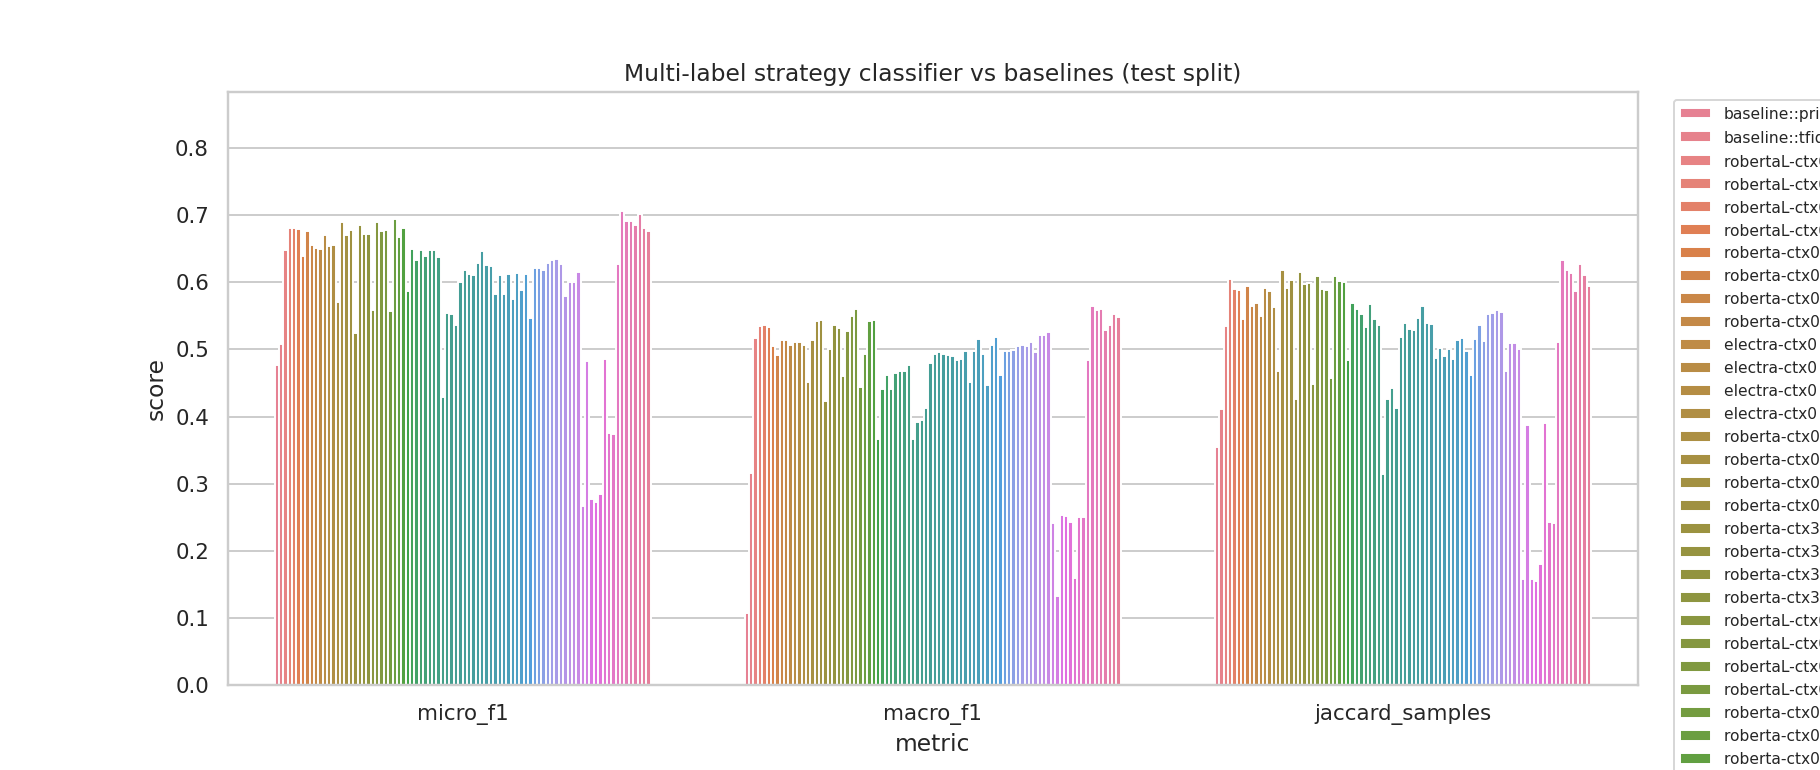
\includegraphics[width=0.82\textwidth]{figures/fig_classifier_comparison.png}
\caption{Micro-F1 across baselines and the final ensemble, category task.}
\label{fig:classifier-comparison}
\end{figure}

\subsection{Per-Category Breakdown and the Rare-Category Gap}

\begin{table}[H]
\centering
\caption{Per-category precision/recall/F1, final system (v17), macro-optimal point, test split.}
\label{tab:per-category}
\begin{tabular}{@{}lrccc@{}}
\toprule
\textbf{Category} & \textbf{Support} & \textbf{Precision} & \textbf{Recall} & \textbf{F1} \\
\midrule
Commitment and Consistency & 22 & 0.147 & 0.227 & 0.179 \\
Urgency and Scarcity & 23 & 0.146 & 0.261 & 0.188 \\
Threat and Pressure & 33 & 0.220 & 0.394 & 0.283 \\
Rational Appeal & 104 & 0.459 & 0.692 & 0.552 \\
Credibility Appeal & 131 & 0.717 & 0.695 & 0.705 \\
Reciprocity and Exchange & 146 & 0.901 & 0.808 & 0.852 \\
Framing and Presentation & 158 & 0.712 & 0.734 & 0.723 \\
Social Influence & 193 & 0.492 & 0.487 & 0.490 \\
Emotional Appeal & 248 & 0.609 & 0.766 & 0.679 \\
Information Provision & 569 & 0.694 & 0.861 & 0.769 \\
Relational and Interactive & 701 & 0.690 & 0.786 & 0.735 \\
\bottomrule
\end{tabular}
\end{table}

\begin{figure}[H]
\centering
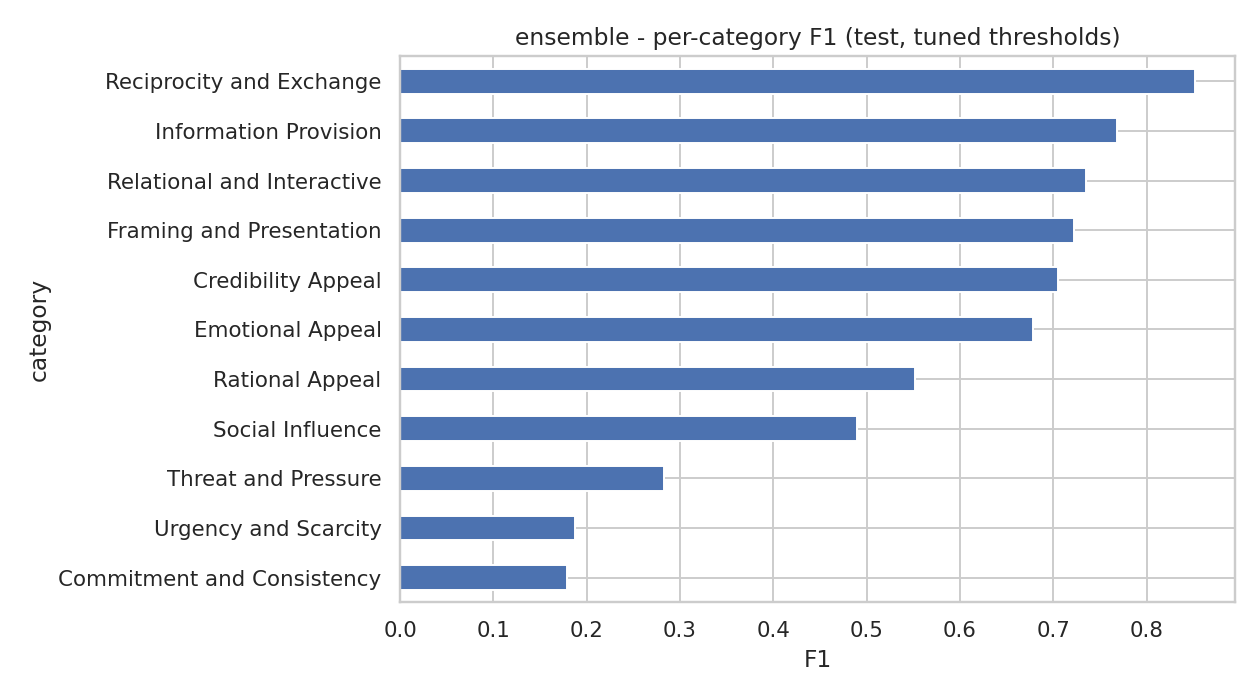
\includegraphics[width=0.85\textwidth]{figures/fig_per_category_f1.png}
\caption{Per-category F1, sorted by support -- the three rarest categories are the visible outliers.}
\label{fig:per-category}
\end{figure}

Table~\ref{tab:per-category} makes the shape of the remaining error obvious:
the three rarest categories (3.4\% of all positive labels in the test split)
score a mean F1 of 0.22, against 0.69 for the other eight. If those three
matched the other eight, overall macro-F1 would be approximately
\textbf{0.68} rather than 0.56 -- essentially the entire remaining gap to a
near-ceiling result is concentrated in these three labels.

This gap is \emph{not} monotonically closing across iterations, and this
report states that plainly rather than only reporting the headline number
that improved. Table~\ref{tab:rare-trajectory} tracks the rare-category mean
F1 against the other eight categories' mean F1 across every category-primary
iteration: the equal-weight multi-task change (v15$\to$v16) improved the
rare categories specifically (the mechanism it was intended to trigger,
Section~\ref{sec:ablation-multitask}), but the subsequent pool change
(v16$\to$v17) improved the \emph{overall} headline by improving the common
eight categories further while the rare three regressed slightly. The
best-ever headline result in Table~\ref{tab:category-headline} is therefore
not evidence that the rare-category problem is solved; it is evidence that a
different lever (encoder pool composition) helps a different part of the
label space, and the rare-category gap remains the right target for future
work (Section~\ref{sec:future-work}).

\begin{table}[H]
\centering
\caption{Rare-category (3 rarest) vs.\ common-category (other 8) mean F1 across iterations,
macro-optimal point.}
\label{tab:rare-trajectory}
\begin{tabular}{@{}lccc@{}}
\toprule
\textbf{Iteration} & \textbf{Rare-3 mean F1} & \textbf{Other-8 mean F1} & \textbf{Overall macro-F1} \\
\midrule
v14 (category auxiliary) & 0.184 & 0.662 & 0.556 \\
v15 (category primary) & 0.201 & 0.680 & 0.549 \\
\textbf{v16 (equal-weight multi-task)} & \textbf{0.237} & 0.681 & 0.560 \\
v17 (+ macro-oriented pool) & 0.216 & \textbf{0.688} & \textbf{0.559} \\
\bottomrule
\end{tabular}
\end{table}

\subsection{Statistical Significance}

\begin{table}[H]
\centering
\caption{Paired significance tests, cluster bootstrap over dialogues, final system (v17).}
\label{tab:significance}
\footnotesize
\begin{tabular}{@{}p{4.0cm}cccp{2.3cm}c@{}}
\toprule
\textbf{Comparison} & \textbf{Point} & \textbf{Metric} & \textbf{$\Delta$} & \textbf{95\% CI} & \textbf{Sig.} \\
\midrule
Ensemble vs.\ best single encoder & micro & micro-F1 & +0.025 & [0.015, 0.034] & \checkmark \\
Ensemble vs.\ best single encoder & macro & macro-F1 & +0.024 & [$-$0.002, 0.049] & $\times$ ($p{=}0.069$) \\
Ensemble vs.\ TF-IDF baseline & micro & micro-F1 & +0.057 & [0.042, 0.072] & \checkmark \\
Ensemble vs.\ TF-IDF baseline & macro & macro-F1 & +0.090 & [0.065, 0.115] & \checkmark \\
micro-opt vs.\ macro-opt point & -- & micro-F1 & +0.015 & [0.008, 0.021] & \checkmark \\
micro-opt vs.\ macro-opt point & -- & macro-F1 & +0.004 & [$-$0.015, 0.022] & $\times$ ($p{=}0.664$) \\
\bottomrule
\end{tabular}
\normalsize
\end{table}

Two results in Table~\ref{tab:significance} are reported precisely because
they complicate the headline story and should not be glossed over. First,
the ensemble's macro-F1 advantage over its single best encoder member is
\emph{not} statistically significant ($p=0.069$) -- the ensembling machinery
(Section~\ref{sec:design-ensemble}) earns a clearly significant micro-F1 gain
and a significant gain over the non-transformer baseline on both metrics,
but its edge over one well-configured transformer on macro-F1 specifically
should be described as suggestive, not established. Second, the
micro-optimal decoding point's macro-F1 is statistically indistinguishable
from the macro-optimal point's macro-F1 ($p=0.664$); part of
Table~\ref{tab:category-headline}'s headline macro-F1 gain over earlier
iterations reflects which candidate a stochastic ensembling search happened
to select, not a real improvement in what the underlying probabilities
encode (Section~\ref{sec:ablation-selection-noise}).

\subsection{Conformal Prediction Sets}
\label{sec:conformal}

As a complementary, distribution-free reliability check, split conformal
prediction \citep{vovk2005conformal} is applied at three target coverage
levels (Table~\ref{tab:conformal}). At 80\% target coverage, empirical
coverage of 0.789 is achieved with a mean prediction-set size of 2.67 labels
(against a true mean cardinality of 1.56) -- the calibration is close to
nominal, and the set-size cost of that calibration is a further, complementary
view of how much genuine per-turn ambiguity the model is carrying, beyond
what a single point-estimate F1 conveys.

\begin{table}[H]
\centering
\caption{Split-conformal prediction coverage, category task, test split.}
\label{tab:conformal}
\small
\begin{tabular}{@{}p{2.2cm}p{2.4cm}p{2.2cm}cc@{}}
\toprule
\textbf{Target coverage} & \textbf{Empirical coverage} & \textbf{Mean set size} & \textbf{Micro-F1} & \textbf{Macro-F1} \\
\midrule
0.90 & 0.878 & 3.75 & 0.526 & 0.454 \\
0.80 & 0.789 & 2.67 & 0.587 & 0.509 \\
0.70 & 0.693 & 2.00 & 0.626 & 0.536 \\
\bottomrule
\end{tabular}
\normalsize
\end{table}

\section{Strategy-Level (41-Way) Results}
\label{sec:strategy-results}

Before the category-first reframing, the strategy-primary line of iterations
peaked at \textbf{micro-F1 0.579, macro-F1 0.350} (micro-optimal) and
\textbf{micro-F1 0.563, macro-F1 0.359} (macro-optimal) at iteration v13 --
the best result achieved under that framing, itself reached by \emph{removing}
four measurably harmful or dominated ensemble members rather than adding
anything (Section~\ref{sec:ablation-summary}). This is retained in this
report both because Module~B's 41-strategy head remains a live output of the
final system (as the secondary/auxiliary head, Section~\ref{sec:category-first})
and because the comparison against Table~\ref{tab:category-headline} is the
direct empirical justification for why the category task became primary: at
its best, the strategy-level macro-F1 (0.359) sits at only 49\% of its own
applicable ceiling (0.733), where the category task's final macro-F1 (0.564)
sits at 71\% of its ceiling (0.793) -- the category task simply has
substantially more learnable headroom.

\section{Decision-Rule Study}
\label{sec:decode-study}

Which of the eleven decision rules (Table~\ref{tab:decision-rules}) should
convert probabilities to label sets is itself fitted on held-out data, never
on the test split. Table~\ref{tab:decode-rules-val} reports every rule's
mean macro-F1 under repeated grouped cross-fitting on the validation split
(4 repeats $\times$ 4 folds, category task, v16 probabilities): the two
empirical-Bayes rules this project contributes rank first and second,
narrowly ahead of the 41-parameter own-threshold rule and comfortably ahead
of the single global threshold and prevalence-anchored rules. Confirmed
against the (never-fitted-to) test split, the same relative ordering holds,
which is itself worth reporting: on the strategy task, an earlier design
iteration found that a 41-parameter rule's validation-set ranking did
\emph{not} reliably predict its test-set behavior (a symptom of
overfitting a validation split as small as 1{,}513 rows), whereas on the
better-supported category task the validation ranking is a trustworthy guide
to test performance.

\begin{table}[H]
\centering
\caption{Decision-rule study, category task, held-out validation (repeated grouped cross-fitting).
Rules marked \textsuperscript{*} are contributed by this project.}
\label{tab:decode-rules-val}
\begin{tabular}{@{}lccc@{}}
\toprule
\textbf{Rule} & \textbf{Val.\ macro-F1} & \textbf{Std.\ dev.} & \textbf{Params} \\
\midrule
\texttt{eb\_shrunk}\textsuperscript{*} & \textbf{0.5646} & 0.0174 & 2 \\
\texttt{eb\_prevalence}\textsuperscript{*} & 0.5645 & 0.0142 & 2 \\
\texttt{perlabel\_ownF1} & 0.5642 & 0.0154 & 41 \\
\texttt{perlabel\_shrunk} & 0.5551 & 0.0173 & 21 \\
\texttt{prevalence} & 0.5431 & 0.0174 & 1 \\
\texttt{global\_micro} (best micro-F1: 0.700) & 0.5249 & 0.0210 & 1 \\
\bottomrule
\end{tabular}
\end{table}

\section{Donation-Outcome Analysis (Module C)}
\label{sec:phase4-results}

Module~C's logistic outcome models are fit on the 1{,}017 annotated
dialogues' \emph{gold} strategy labels. Table~\ref{tab:phase4} reports each
model's cross-validated pseudo-$R^2$ alongside its in-sample figure, which is
consistently and substantially higher -- a direct illustration of why the
out-of-sample figure, not the in-sample one, is the number to trust with up
to 28 features fit on 1{,}017 observations.

\begin{table}[H]
\centering
\caption{Donation-outcome logistic models (McFadden pseudo-$R^2$), gold labels.}
\label{tab:phase4}
\begin{tabular}{@{}p{5.2cm}cccc@{}}
\toprule
\textbf{Model} & \textbf{Features} & \textbf{In-sample $R^2$} & \textbf{CV $R^2$} & \textbf{CV std.} \\
\midrule
M1: 11 categories & 11 & 0.140 & 0.116 & 0.036 \\
M2: M1 + sentiment/interest & 13 & 0.188 & 0.157 & 0.038 \\
M3: guilt $\times$ reciprocity + sent./interest & 4 & 0.064 & 0.056 & 0.024 \\
M4: M1 + co-occurrence + richness & 28 & 0.224 & \textbf{0.165} & 0.046 \\
\bottomrule
\end{tabular}
\end{table}

\begin{figure}[H]
\centering
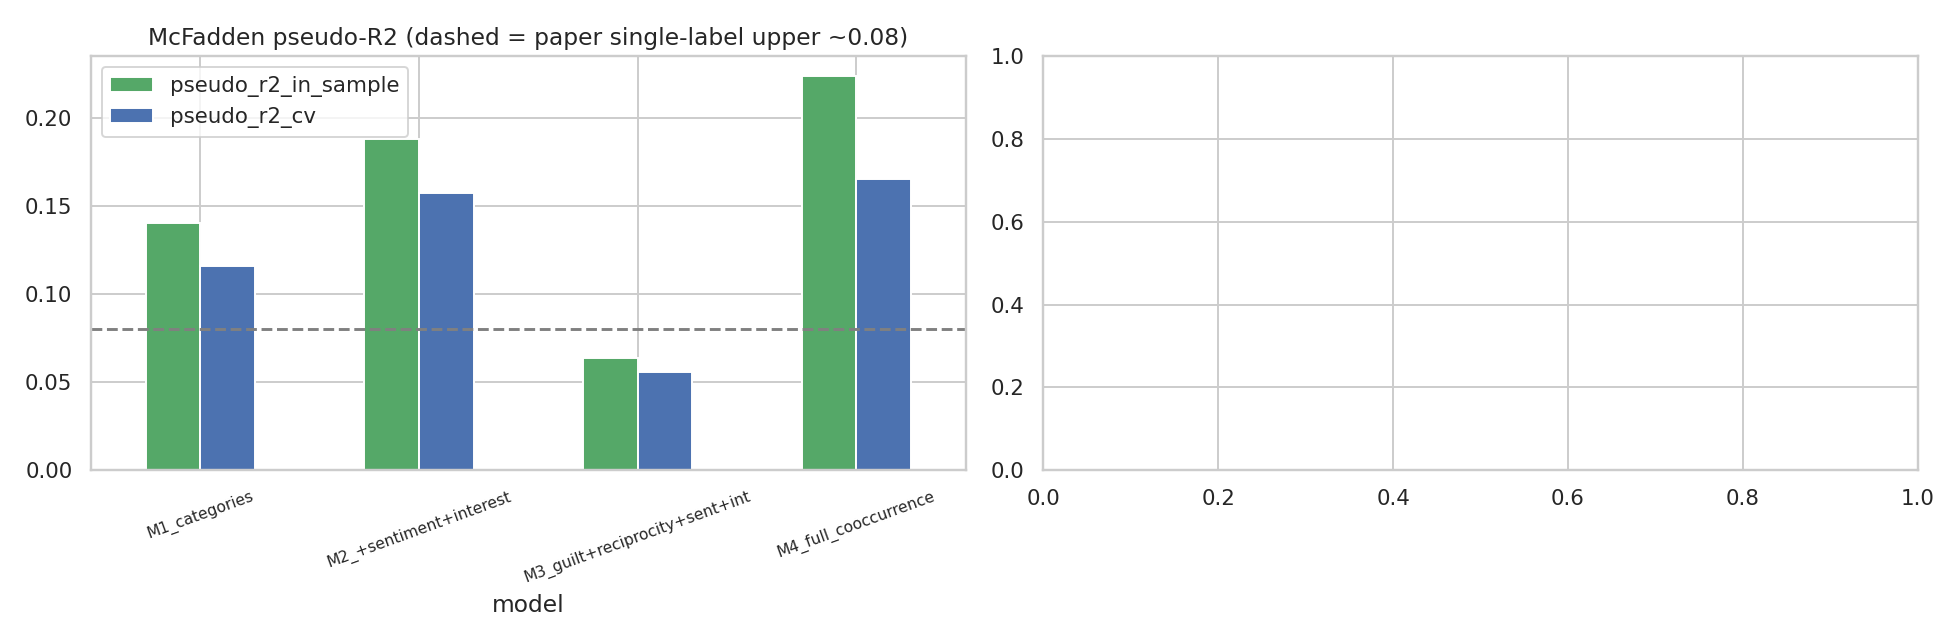
\includegraphics[width=0.8\textwidth]{figures/fig_phase4.png}
\caption{Donation-outcome model diagnostics (Module C).}
\label{fig:phase4}
\end{figure}

M4's cross-validated pseudo-$R^2$ of 0.165 is roughly double the 0.015--0.08
range the team's prior working notes recorded for a single-label
specification of a related outcome-modeling task \citep{petrova_singlelabel}.
This project treats that specific comparison with caution and states the
reason explicitly: the two settings differ in labeling scheme, in the
outcome variable definition, \emph{and} in feature count simultaneously, so
the improvement cannot be attributed to multi-labeling alone from this
comparison. To isolate the multi-labeling question specifically, a
single-label \emph{projection} of this project's own gold data is fit under
the identical M1--M4 specification, holding the corpus, the outcome
definition, and the feature-construction code fixed and changing only
whether a turn may carry one label or several. Under this controlled
comparison, multi-label M4 reaches a cross-validated pseudo-$R^2$ of 0.165
against 0.133--0.138 for the best single-label projection (commonest-label,
rarest-label, and five-seed-random-label projection rules), a genuine
\textbf{+0.03} advantage for multi-labeling that survives every projection
rule tried -- the honest, narrowly-scoped version of the multi-label claim,
in contrast to the roughly $+0.15$ that the uncontrolled cross-paper
comparison would suggest.

\subsection{Category--Donation Associations}

\begin{table}[H]
\centering
\caption{Category odds ratios for donation outcome, M1 (gold labels, significant at $p<0.01$ in bold).}
\label{tab:odds-ratios}
\begin{tabular}{@{}lccc@{}}
\toprule
\textbf{Category} & \textbf{Coefficient} & \textbf{Odds Ratio} & \textbf{$p$-value} \\
\midrule
Reciprocity and Exchange & \textbf{1.575} & \textbf{4.83} & \textbf{$<$0.001} \\
Threat and Pressure & \textbf{$-$0.927} & \textbf{0.40} & \textbf{$<$0.001} \\
Information Provision & \textbf{1.082} & \textbf{2.95} & \textbf{0.001} \\
Emotional Appeal & 0.231 & 1.26 & 0.183 \\
Social Influence & 0.208 & 1.23 & 0.200 \\
Framing and Presentation & 0.147 & 1.16 & 0.362 \\
Credibility Appeal & 0.105 & 1.11 & 0.511 \\
Urgency and Scarcity & 0.143 & 1.15 & 0.584 \\
Relational and Interactive & $-$0.191 & 0.83 & 0.651 \\
Rational Appeal & 0.030 & 1.03 & 0.854 \\
Commitment and Consistency & 0.008 & 1.01 & 0.972 \\
\bottomrule
\end{tabular}
\end{table}

Dialogues that use reciprocity-based appeals (e.g. emphasizing the mutual
benefit of donating) have nearly \textbf{5$\times$} the odds of ending in a
donation, controlling for the other ten categories; dialogues that lean on
threat-and-pressure tactics have well under half the odds. Two further
richness measures confirm the same direction with non-parametric tests: a
Mann--Whitney comparison of donated vs.\ non-donated dialogues finds
significantly more distinct strategies (mean 9.64 vs.\ 8.56, $p<0.001$),
more distinct categories (5.97 vs.\ 5.33, $p<0.001$), and more total
strategy instances (17.95 vs.\ 16.32, $p<0.001$) in dialogues that end in a
donation. A prior single-label analysis of a related corpus reported a mean
of only 4--5 distinct strategies per dialogue \citep{petrova_singlelabel};
this project's multi-label annotation recovers a mean of \textbf{9.34}, a
direct consequence of allowing a turn to carry more than one simultaneous
label rather than a difference in persuader behavior.

\subsection{A Limitation Stated Explicitly: Temporal Direction}

The odds ratios in Table~\ref{tab:odds-ratios} are estimated from a
bag-of-strategies representation of each dialogue and therefore cannot
distinguish a strategy that \emph{causes} donation from a strategy that is a
\emph{reaction to} an already-forming decision. This project's own working
notes flag a concrete instance: gratitude-expressing strategies occur
disproportionately late in a dialogue, and a preliminary position-windowed
check found that roughly two-thirds of a large raw gratitude-donation
association in earlier project notes disappeared once only gratitude
expressed \emph{before} the point where the persuadee could plausibly have
already committed was counted -- consistent with a persuader thanking a
donor \emph{after} they agree, rather than gratitude persuading them to
agree. This project reports that finding as a scope boundary rather than
resolving it here: the position-windowed check used a quick, single-strategy-
at-a-time comparison with small per-window sample sizes and is not presented
in Table~\ref{tab:odds-ratios} or treated as a validated result. The
temporal, commitment-turn-aware hazard-model analysis needed to resolve it
rigorously is named as future work (Section~\ref{sec:future-work}) rather
than included here, precisely so that Table~\ref{tab:odds-ratios} is not
overstated as more causally interpretable than an observational, un-randomized
corpus of this size can actually support.

\section{Ablation Study}
\label{sec:ablation-summary}

Table~\ref{tab:ablation-summary} consolidates every controlled intervention
tested across the project's seventeen design iterations. Each row is a
single, isolated change measured against a sentinel-verified baseline
(Section~\ref{sec:design-methodology}); ``Verdict'' records whether the
change was kept in the final system.

\begin{table}[H]
\centering
\footnotesize
\caption{Consolidated ablation record. $\Delta$mi / $\Delta$ma are the measured change in
micro-F1 / macro-F1 for that specific, isolated intervention.}
\label{tab:ablation-summary}
\begin{tabular}{@{}p{3.7cm}p{1.3cm}p{3.3cm}rrp{2.2cm}@{}}
\toprule
\textbf{Intervention} & \textbf{Task} & \textbf{Member(s)} & \textbf{$\Delta$mi} & \textbf{$\Delta$ma} & \textbf{Verdict} \\
\midrule
Target-span attention pooling & Strategy & ctx1 pair & +0.002 & $-$0.007 & Rejected (underpowered) \\
Target-span pooling, retest & Strategy & ctx3 pair & $-$0.008 & +0.010 & Rejected (a trade) \\
Prior-initialized head bias & Strategy & 1 member & $-$0.008 & $-$0.012 & Rejected (harmful) \\
Context width 0$\to$3 (dialogue-pretrained enc.) & Strategy & TOD-BERT & +0.028 & +0.017 & \textbf{Adopted} \\
Context width 0$\to$3 (general enc.) & Strategy & RoBERTa & $-$0.005 & +0.022 & \textbf{Adopted} \\
Context width 0$\to$3 (3rd architecture) & Strategy & ELECTRA & $-$0.001 & $-$0.039 & Rejected (architecture-specific) \\
DB-rebalanced loss weighting & Strategy & ELECTRA & +0.009 & $-$0.007 & Kept, micro-members only \\
EDA augmentation on/off & Strategy & RoBERTa & +0.014 & $-$0.009 & Split, macro-members off \\
Pruning by ensemble-blend weight & -- & -- & n/a & n/a & \textbf{Rejected} (weights not reproducible) \\
Category as primary task & Category & full pool & +0.001 & $-$0.007 & Neutral alone \\
Equal-weight multi-task loss & Category & full pool & +0.001 & \textbf{+0.009} & \textbf{Adopted} \\
Context width 0$\to$3 & Category & 4-member set & +0.005 & $-$0.005 & Rejected (no macro gain) \\
Macro-oriented pool expansion & Category & +2 members & +0.006 & +0.018 & \textbf{Adopted} (best-ever) \\
\bottomrule
\end{tabular}
\end{table}

\subsection{Selection Noise: a Methodological Caution}
\label{sec:ablation-selection-noise}

A negative-space finding is reported here on equal footing with the positive
ones, because it changed how every later iteration was evaluated. Running an
identical configuration twice (on two independent Kaggle accounts,
Section~\ref{sec:design-methodology}) produced ensemble-blend weights that
differed by up to 2.7$\times$ between the two runs for the same member, with
one member receiving zero weight in one run and non-trivial weight in the
other. The stochastic bagged-greedy search that selects the final ensemble
blend is simply not a reproducible enough quantity to prune members by:
doing so would be pruning on noise, the same failure mode this project
guards against when selecting a decision rule (Section~\ref{sec:decode-study}).
Every pruning decision in Table~\ref{tab:ablation-summary} is instead based
on deterministic \emph{member-level} scores, which reproduce to four decimal
places (Section~\ref{sec:design-methodology}).

\subsection{Context Width: an Architecture-Dependent Effect}
\label{sec:ablation-context}

Whether giving an encoder more preceding dialogue turns as context helps is
not a single, corpus-wide answer -- it depends on the encoder's own
pretraining, and had to be measured per architecture rather than assumed.
Extending the context window from 0 to 3 preceding turns (strategy task,
Table~\ref{tab:ablation-summary}) helped TOD-BERT substantially on both
metrics ($+0.028$ micro / $+0.017$ macro) and helped RoBERTa on macro-F1
specifically ($-0.005$ micro / $+0.022$ macro), but measurably \emph{hurt}
ELECTRA ($-0.001$ micro / $-0.039$ macro). TOD-BERT is pretrained
specifically on task-oriented dialogue \citep{wu2020todbert}, which is the
most plausible explanation for why it is the one encoder that reliably turns
additional context into signal; ELECTRA has no such dialogue-specific
pretraining and its discriminative replaced-token objective may be
comparatively more sensitive to the added, potentially distracting, context
tokens. On the category task specifically, the same intervention (applied to
a four-member subset of the pool) was re-measured and found \emph{not} to
help macro-F1 at all ($-0.005$), a task-specific null result reported
alongside the strategy-task positive one precisely because the two tasks
disagree, and assuming an effect measured on one task transfers to the other
would have been an error.

\subsection{Augmentation and Rebalancing: a Trade, Not a Fix}
\label{sec:ablation-augmentation}

The EDA rare-class augmentation (Section~\ref{sec:design-augmentation}) was
built to help macro-F1 -- more copies of a turn carrying a rare strategy
should mean more gradient signal for that strategy. Measured in isolation,
it does the opposite: $+0.014$ micro-F1 but $-0.009$ macro-F1 on the same
member. The mechanism, diagnosed directly from the corpus rather than
inferred from the result alone: oversampling a turn to help its rare
strategy also oversamples whichever \emph{common} strategies happen to
co-occur on that same turn (Section~\ref{ch:research}), so a strategy
intended to receive a 9$\times$ boost receives it, but every common
co-occurring strategy receives an unintended $\sim$1.5$\times$ boost as a
side effect -- roughly a third of the intended rebalancing is spent
inflating labels that were already abundant. Distribution-Balanced
rebalanced loss weighting \citep{wu2020distribution}, which damps a common
label's loss contribution specifically on turns it is riding alongside a
rare label, shows the identical micro-positive/macro-negative pattern
($+0.009$/$-0.007$) via a different mechanism (precision recovery on the
common labels, rather than more signal for the rare ones). Both findings
point the same direction and motivated the final design's objective-split
principle (Section~\ref{sec:objective-split}): each intervention is a
genuine trade between the two metrics, so rather than picking one setting
for the whole ensemble, micro-oriented members keep augmentation on and add
DB-rebalancing, and macro-oriented members turn augmentation off and rely on
positive-class weighting instead.

\subsection{Equal-Weight Multi-Task Loss: Mechanism Check}
\label{sec:ablation-multitask}

The equal-weight multi-task change (raising the auxiliary strategy head's
loss weight from 0.3 to 1.0, category task, Table~\ref{tab:ablation-summary})
is the one intervention in this study whose effect was verified against a
specific, falsifiable mechanism rather than reported as a bare number: it
was hypothesized to help specifically because the fine-grained 41-strategy
gradient should regularize hardest exactly where category-level supervision
alone is weakest -- the three rarest categories, each built from strategies
that are themselves individually rare. Table~\ref{tab:rare-trajectory}
confirms this directly: the rare-3 mean F1 rose from 0.201 to 0.237 while
the common-8 mean stayed flat (0.680$\to$0.681) across this specific change,
which is the pattern the mechanism predicts and not the pattern a generic
regularization effect (which would move both groups together) would produce.

\section{Module A: Donation-Intent Classification}
\label{sec:module-a-results}

\begin{table}[H]
\centering
\caption{Donation-intent classification (Module A), binary task, test split.}
\label{tab:module-a}
\begin{tabular}{@{}lcc@{}}
\toprule
\textbf{Model} & \textbf{Accuracy} & \textbf{Macro-F1} \\
\midrule
Majority-class baseline & 72.5\% & 0.421 \\
Flat single-stream baseline (earliest iteration) & -- & $\approx$0.63 \\
Hierarchical + specialist routing (intermediate) & -- & 0.834 \\
\textbf{Dual-stream cross-attention (final, v14-Antiphony)} & \textbf{89.5\%} & \textbf{0.862} \\
\bottomrule
\end{tabular}
\end{table}

Module~A's final architecture encodes the persuader's and persuadee's turns
as separate role-pure streams and applies directional cross-attention
between them before a trajectory-tracking recurrent layer
(Section~\ref{sec:design-module-a}). Every backbone tested (RoBERTa,
DeBERTa-v3, TOD-BERT) improved when moved from a flat single-stream encoding
to this dual-stream design, indicating the gain is attributable to the
architecture rather than to any one pretrained encoder.

\section{Module D: Cross-Domain Generalization}
\label{sec:generic-results}

\begin{table}[H]
\centering
\caption{Module A's architecture retrained on the generic buyer--seller negotiation domain
(500 dialogues, binary outcome), test split.}
\label{tab:generic}
\begin{tabular}{@{}lcc@{}}
\toprule
\textbf{Backbone} & \textbf{Accuracy} & \textbf{Macro-F1} \\
\midrule
Majority-class baseline & 53.3\% & 0.348 \\
TOD-BERT & 92.0\% & 0.920 \\
RoBERTa-base & 93.3\% & 0.933 \\
\textbf{DeBERTa-v3-base} & \textbf{97.3\%} & \textbf{0.973} \\
\bottomrule
\end{tabular}
\end{table}

The same dual-stream architecture, retrained without domain-specific
modification on a structurally similar but topically distinct
buyer--seller price-negotiation corpus, reaches 97.3\% accuracy with its
strongest backbone -- evidence that the architectural gain measured in
Module~A (Table~\ref{tab:module-a}) is a property of the dual-stream design
applied to two-party persuasive dialogue in general, and not an artifact
specific to the donation-solicitation domain or to this particular corpus.

\section{Summary}

Across all four modules, the results in this chapter support three
higher-level conclusions that carry into Chapter~\ref{ch:conclusion}: (i)
evaluating a classifier against its corpus's own measured annotation
ceiling, rather than against 1.0, changes which results should be considered
successes -- the final category-level micro-F1 of 0.706 is close to that
ceiling and should be read accordingly; (ii) a disciplined, hypothesis-driven,
sentinel-verified experimental protocol is what makes it possible to tell a
real effect (context width for a dialogue-pretrained encoder) from a
plausible-sounding one that measurably fails (target-span pooling,
prior-initialized biases) or a genuine trade rather than a free improvement
(augmentation, class-imbalance reweighting); and (iii) the remaining error
is not evenly distributed -- it is concentrated in three rare categories
that the strongest single lever found so far (equal-weight multi-task
supervision) helps, but does not solve, leaving a clearly scoped target for
future work.
